\appendix

\phantomsection
\section*{Appendices}
\addcontentsline{toc}{section}{Appendices}
\renewcommand{\thesubsection}{\Alph{subsection}}

\label{annex:framework}

\subsection{Inter-dependencies for the "Physical Basic Structure" \label{annex:phy-bas-struc}}

\begin{figure}[h]
    \centering
    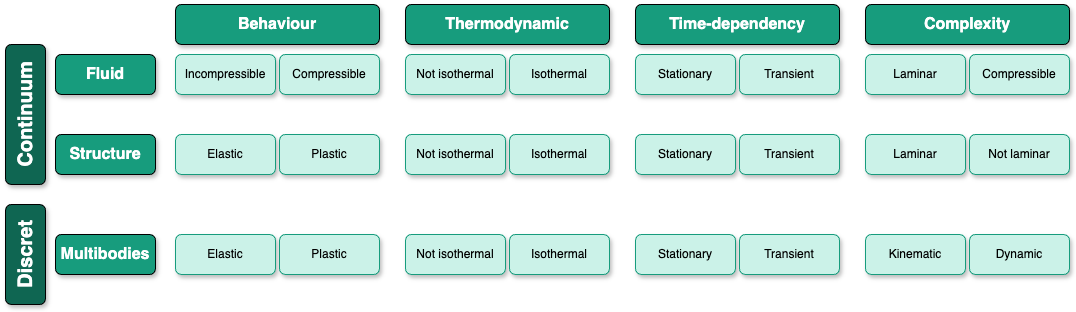
\includegraphics[width=\textwidth]{images/Concept-PhysicalInterdependencies.drawio.png}
    \caption{\label{fig:phy-bas-struc}  Inter-Dependencies for the "Physical Basic Structure" \cite{assistSim}}
\end{figure}


\subsection{Screenshot of Excel File Used to Import Examples into the Knowledge graph\label{annex:screen-excel}}

\begin{figure}[h]
    \centering
    \frame{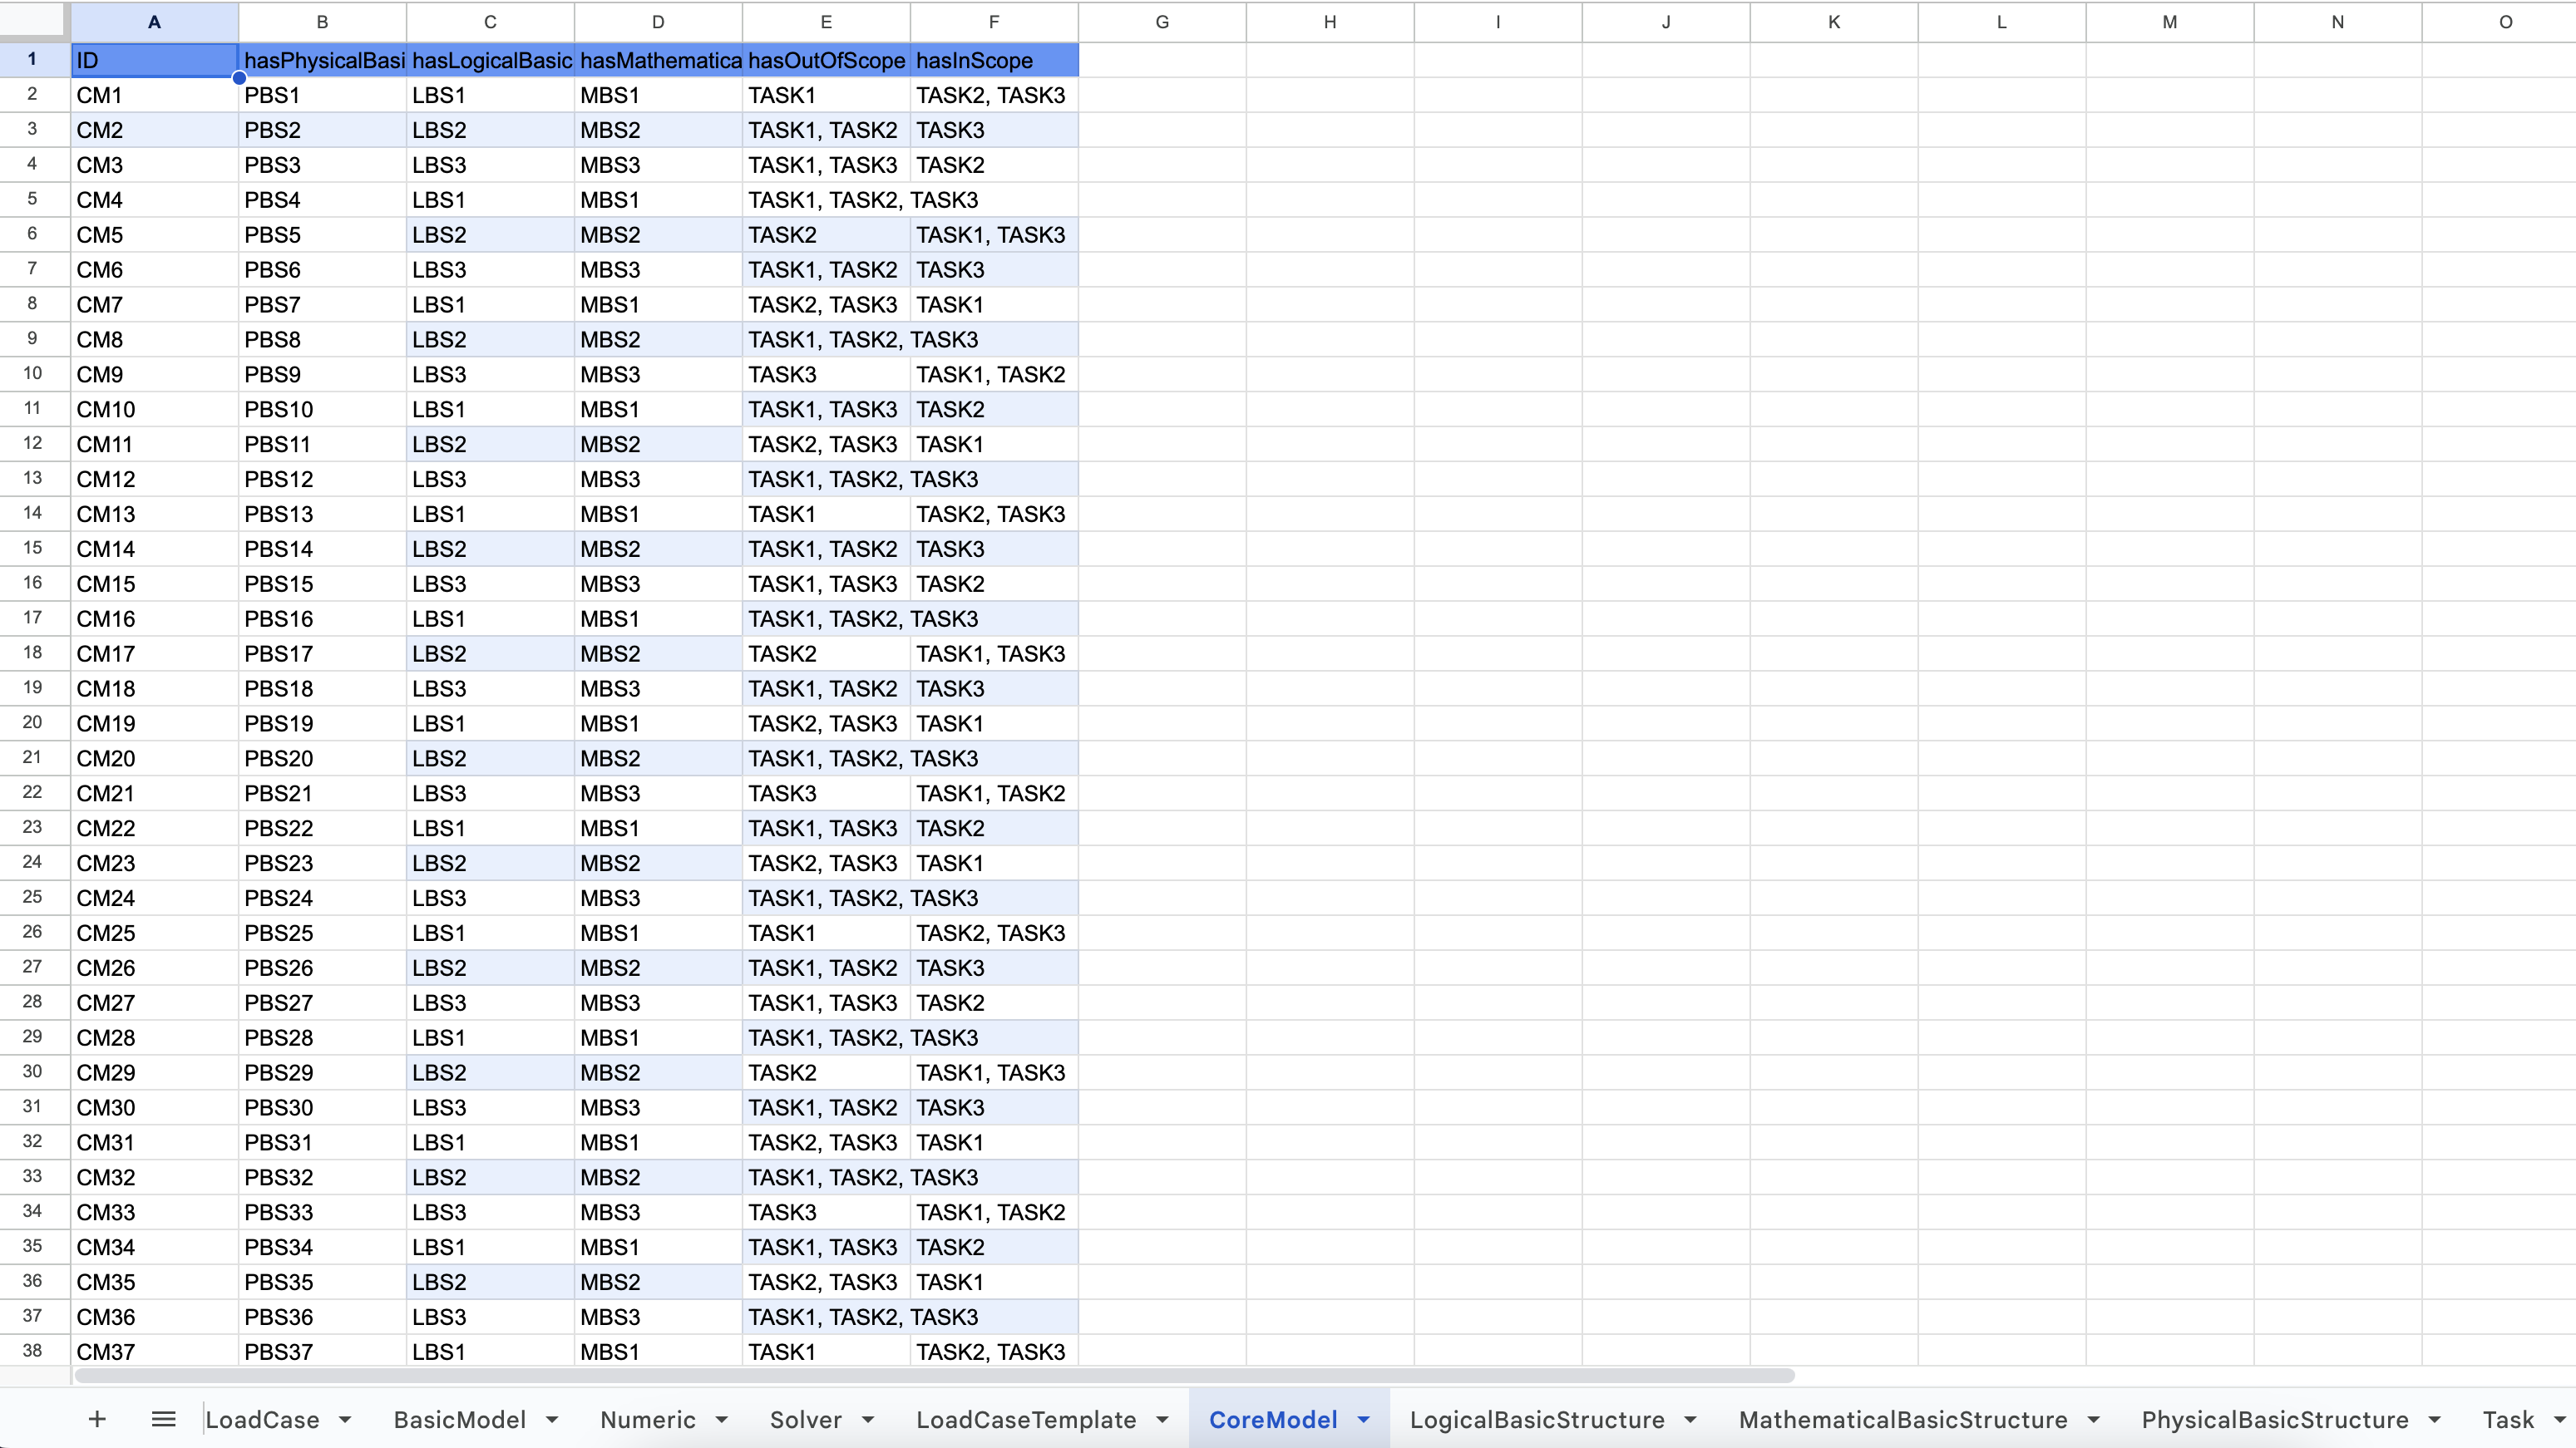
\includegraphics[width=\textwidth]{images/loadcase-excell.png}}
    \caption{\label{fig:screen-excel} Screenshot of Excel File Used to Import Examples into the Knowledge Graph}
\end{figure}



\clearpage
\subsection{Function to Create the Schema of the Ontology (Full)\label{annex:create-schema-full}}

\begin{lstlisting}[language=Python, caption=Function to Create the Schema of the Ontology (Full), label={lst:create-schema-full}]
def create_schema_from_class(
        self, class_uri: str, depth: int, visited: dict[str, bool]
    ) -> Node:
        visited[class_uri] = True
        node = Node(None, class_uri, depth)

        # Get all DataProperties of the instance
        data_properties = get_class_data_properties(class_uri)
        # Get all DataProperties of the superClass
        super_data_properties = get_super_class_data_properties(class_uri)
        data_properties += super_data_properties

        # Add all data properties to the node
        for property_uri, type_uri, type_list in data_properties:
            property_suffix_uri = extractSuffixURI(Config.BASEPREFIX, property_uri)
            type = type_list if type_list else extractSchemaType(type_uri)
            node.addAttribute(DataObject(property_suffix_uri, None, type, depth))

        # Get all ObjectProperties of the instance
        object_properties = get_class_object_properties(class_uri)
        # Get all ObjectProperties of his super class
        super_object_properties = get_super_class_object_properties(class_uri)
        object_properties += super_object_properties

        # Add edges
        for property_uri, child_class_name_uri in object_properties:
            child_class_name_turtle_uri = extractSuffixURI(
                Config.BASEPREFIX, child_class_name_uri
            )
            # Check if the class is not already visited and is not in the list of excluded classes
            if (child_class_name_turtle_uri not in visited) and (
                child_class_name_turtle_uri not in Config.EXCLUDED_CLASSES
            ):
                property_suffix_uri = extractSuffixURI(Config.BASEPREFIX, property_uri)
                node.addEdge(
                    property_suffix_uri,
                    self.create_schema_from_class(
                        child_class_name_turtle_uri, depth + 1, visited
                    ),
                )

        return node
\end{lstlisting}



\clearpage
\subsection{Function to Find the Similarity Between one Case and all the Cases in the Data-Base (Full)\label{annex:comp-sim-full}}

\begin{lstlisting}[language=Python, caption=Function to Find the Similarity Between One Case and All the Cases in the Data-Base (Full), label={lst:comp-sim-full}]
def computeSimilarity(
        self, target: Node, mandatories: list[str], responsesStack: dict[str, Any]
    ) -> list[Similarity]:
        similarities = []

        for graphKey, graph in self.ontology.graphs.items():
            # Check if the graph respect the mandatories
            check = checkValidGraphByMandatories(graph, mandatories, responsesStack)
            if check:
                simi = Similarity(self.computeSimilarityForNode(graph, target), graph)
                similarities.append(simi)

        mean = self.similarityMean(similarities)

        similarities = list(filter(lambda x: x.value >= mean, similarities))

        # order by similarity descending
        similarities.sort(key=lambda x: x.value, reverse=True)

        return similarities
\end{lstlisting}



\clearpage
\subsection{Function to Find the Similarity Between two Cases (Full)\label{annex:comp-sim-node-full}}

\begin{lstlisting}[language=Python, caption=Function to Find the Similarity Between Two Cases (Full), label={lst:comp-sim-node-all}]
# compute similarity between two graph using local to global traversal
    def computeSimilarityForNode(self, node: Node, target: Node) -> float:
        # Local computation
        attributSimilarity = 0
        numberOfAttribute = 0
        for key, targetAttribute in target.attributes.items():
            if targetAttribute.value is not None:
                nodeAttribute = node.getAttribute(key)

                if nodeAttribute is None:
                    continue

                sim = self.computeSimilarityForAttribute(nodeAttribute, targetAttribute)
                attributSimilarity += sim
                numberOfAttribute += 1

        # Global computation
        childSimilarity = 0
        numberOfEdges = 0
        for key, targetEdges in target.edges.items():
            nodeEdges = node.getEdge(key)

            if nodeEdges is None:
                continue

            # iterate over all the edeges of this node with the same URI
            collectorSim = [0]
            for targetEdge in targetEdges:
                for nodeEdge in nodeEdges:
                    if nodeEdge is not None:
                        collectorSim.append(
                            self.computeSimilarityForNode(
                                nodeEdge["childNode"], targetEdge["childNode"]
                            )
                        )

            sim = max(collectorSim)
            childSimilarity += sim
            numberOfEdges += 1

        if (numberOfAttribute + numberOfEdges) == 0:
            return 0

        nodeSimilarity = (attributSimilarity + childSimilarity) / (
            numberOfAttribute + numberOfEdges
        )

        return nodeSimilarity
\end{lstlisting}


\clearpage
\subsection{Function to Compute the Similarity Value Between two Attributes (Full)\label{annex:comp-sim-att-full}}
\begin{lstlisting}[language=Python, caption=Function to Compute the Similarity Value Between Two Attributes, label={lst:comp-sim-att}]
def computeSimilarityForAttribute(
        self, nodeAttribute: DataObject, targetAttribute: DataObject
    ) -> float:
        similarity = 0

        match nodeAttribute.type:
            case "string":
                similarity = computeStringLevensteinSimilarity(
                    nodeAttribute.value, targetAttribute.value
                )
            case "int":
                similarity = computeNumericSigmoidSimilarity(
                    nodeAttribute.value, targetAttribute.value
                )
            case "double":
                similarity = computeNumericSigmoidSimilarity(
                    nodeAttribute.value, targetAttribute.value
                )
            case "decimal":
                similarity = computeNumericSigmoidSimilarity(
                    nodeAttribute.value, targetAttribute.value
                )
            case "float":
                similarity = computeNumericSigmoidSimilarity(
                    nodeAttribute.value, targetAttribute.value
                )
            case "boolean":
                similarity = self.computeEqualSimilarity(
                    nodeAttribute.value, targetAttribute.value
                )
            case "date":
                similarity = computeStringSortRatio(
                    nodeAttribute.value, targetAttribute.value
                )
            case _:
                similarity = self.computeEqualSimilarity(
                    nodeAttribute.value, targetAttribute.value
                )

        return similarity
\end{lstlisting}